\documentclass[12pt]{article}
\usepackage{tabularx} % extra features for tabular environment
\usepackage{amsmath}  % improve math presentation
\usepackage{graphicx} % takes care of graphic including machinery
\usepackage[margin=1in,letterpaper]{geometry} % decreases margins
\usepackage{cite} % takes care of citations
\usepackage[final]{hyperref} % adds hyper links inside the generated pdf file
\hypersetup{
	colorlinks=true,       % false: boxed links; true: colored links
	linkcolor=blue,        % color of internal links
	citecolor=blue,        % color of links to bibliography
	filecolor=magenta,     % color of file links
	urlcolor=blue         
}
\usepackage{blindtext}
\usepackage{float}
\usepackage[brazil]{babel}   
%++++++++++++++++++++++++++++++++++++++++


\begin{document}

\title{Relatório Técncio - Análise CFD de tubulação cilíndrica.}
\author{Fernando Barroso Vasconcelos Mendes}
\date{\today}
\maketitle

\begin{abstract}
A dinâmica dos fluidos computacional é um ramo da engenharia que se utiliza de recursos computacionais para obter resultados numéricos decorrentes das equações físicas da mecânica dos fluidos. Este relatório faz uma análise de uma tubulação cilíndrica simples, a partir de dados experimentais, com o objetivo de verificar se há problemas de operação e entender o comportamento do escoamento no interior da tubulação. Desse modo, os principais dados utilizados foram a vazão volumétrica e a perda de carga na tubulação. Além disso, é incluído a fundamentação teórica que rege o escoamento para nortear a simulação computacional. Por fim, conclui-se que existem problemas na tubulação ou nas medições realizadas.
\end{abstract}


\section{Introdução}


O principal objetivo do projeto é realizar um estudo numérico de uma instalação de bombeamento de água. Uma seção de tubulação de 1 metro de comprimento e 40 mm de diâmetro tem apresentado problemas. A perda de carga foi medida usando sensores de pressão, e mensurou-se uma queda de pressão de 2 Pa. A bomba que supre esta tubulação com água está operando em potência máxima. Também se mediu a vazão deste escoamento, obtendo um valor de 0,0001 metro cúbico por segundo na saída do tubo.

A ferramenta de simulação escolhida para a realização do estudo é o Ansys CFX, pois mostra-se como código comercial adequado ao cenário a ser estudado. A finalidade do projeto é acadêmica, isto é, visa prover um conhecimento extra à disciplina de Dinâmica dos Fluidos por meio do uso de Dinâmica dos Fluidos Computacional (CFD).

Desse modo, alguns requisitos de solução são estabelecidos para que a análise seja realizada com o devido embasamento visando minimizar possíveis erros. Logo, cabe citar a determinação da vazão volumétrica na saída da tubulação, a determinação da perda de carga e a determinação da tensão cisalhante na parede.



\section{Desenvolvimento}

Na seção \ref{mm}, será explicado o procedimento para atingir os objetivos, como serão realizados os cálculos e simulações. Em seguida, no tópico \ref{resultados}, serão mostrados os cálculos, resultados de simulações e análise desses resultados.
\subsection{Materiais e Métodos}
\label{mm}
Antes de iniciar qualquer tipo de simulação é imprescindível atentar-se para o fenômeno físico em si visando avaliar quais hipóteses de simplificação podem ser aplicadas no cenário. Adotar ou não essas hipóteses estão relacionadas com a influência nos parâmetros a serem analisados, a precisão necessária nos resultados, o poder computacional envolvido e o tempo disponível para realização do estudo.
Neste projeto, tendo em vista as considerações feitas, as seguintes hipóteses serão adotadas: 
\begin{itemize}
	\item Escoamento incompressível;
	\item Escoamento plenamente desenvolvido;
	\item A rugosidade do material da tubulação é desprezível;
	\item A tubulação não apresenta flanges;
	\item A troca de calor é desprezível.
\end{itemize}

Desse modo, para realizar a simulação será usado o software comercial Ansys Workbench 19.2, a geometria do problema usará o SpaceClaim, ferramenta de modelagem 3D do Ansys já incorporada ao Workbench 19.2, como solver adotar-se-á o CFX, no qual também é possível realizar o pós-processamento.

Além disso, visando facilitar a visualização dos dados, a pressão relativa na saída do tubo será considerada igual a 0, pois o interesse principal está na determinação da perda de carga e não no valor exato da pressão absoluta. 

A etapa de pré-processamento foi realizada conforme as grandezas físicas calculadas teoricamente, nessa etapa foram estabelecidas condições de velocidade e pressão no domínio de simulação (condições de contorno) e parâmetros particulares do software. O poder de processamento é algo preponderante para os prazos de estudo numérico computacional de dinâmica dos fluidos, portanto, nesse contexto, em grandes projetos é comum usar-se clusters, comumente conhecidos como supercomputadores. No entanto, para esse projeto não se dispõe de tamanha capacidade computacional. 

Por fim, em um projeto de CFD, a precisão necessária é um ponto importante, pois impactará diretamente na qualidade e quantidade dos elementos de malha, no poder de processamento necessário e no tempo de simulação. Logo, para esta análise adotar-se-á precisão condizente com o necessário em uma indústria, tendo em vista o viés educacional do estudo, a tolerância entre o teórico e o numérico não deve exceder 10\%.

\subsection{Resultados}
\label{resultados}
\subsubsection{Teóricos}
O problema estudado fornece a vazão volumétrica de água na tubulação, então, tendo em vista que a área da tubulação é constante, pode-se determinar a velocidade de escoamento utilizando a equação \ref{eq:vazao}.
\begin{equation}
v=\frac{\dot{V}}{A} \rightarrow v=0,0795 \mathrm{m} / \mathrm{s}
\label{eq:vazao}
\end{equation}

O próximo passo é a determinação do número de Reynolds, coeficiente adimensional que relaciona as forças inerciais com as forças de viscosidade, por meio da equação \ref{eq:reynolds}, onde $\rho_{w} = 997 kg/m^3$, $\mu_{w} = 0.89$ $10^-3 kg/m.s$.

\begin{equation}
R e = \frac{\rho_{\text {w}} v d}{\mu_{\text {w}}} \rightarrow R e=3565
\label{eq:reynolds}
\end{equation}

Desse modo, o número de Reynolds $Re$ indica um escoamento de transição entre o laminar e o turbulento \cite{cengel}, tal fato é relevante para configuração adequada do software. Portanto, a queda de pressão nesse contexto é dada pela equação \ref{eq:qpressao}.
\begin{equation}
\Delta P_{L, T} = f \frac{L}{d} \frac{\rho_{\text {w}} v^{2}}{2}
\label{eq:qpressao}
\end{equation}
Por fim, é necessário estimar o fator de atrito $f$ por meio do Diagrama de Moody, porém, caso necessário, pode-se determiná-lo por meio da equação de Prandtl. Após consultar o Diagrama, o fator foi estimado em $f = 0.042$. Aplicando os valores determinados anteriormente na equação \ref{eq:qpressao} encontra-se $\Delta P_{L,T} = 3.31 Pa$.


\subsubsection{Numéricos}

A geometria a ser estudada representa a região de escoamento plenamente desenvolvido que se situa imediatamente após o comprimento de entrada, região caracterizada por um fluxo não uniforme, vide Fig. \ref{fig:schematics}. Em seguida,apresenta-se a geometria da tubulação construída no SpaceClaim, conforme as dimensões especificadas, na Fig. \ref{fig:isometric}.


\begin{figure}[H]
    \centering
    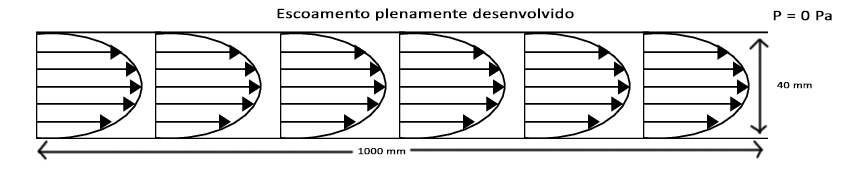
\includegraphics[width=.6\textwidth]{fig/schematics.png}
    \caption{Esquemático da geometria.}
		\label{fig:schematics}
\end{figure}

\begin{figure}[H]
    \centering
    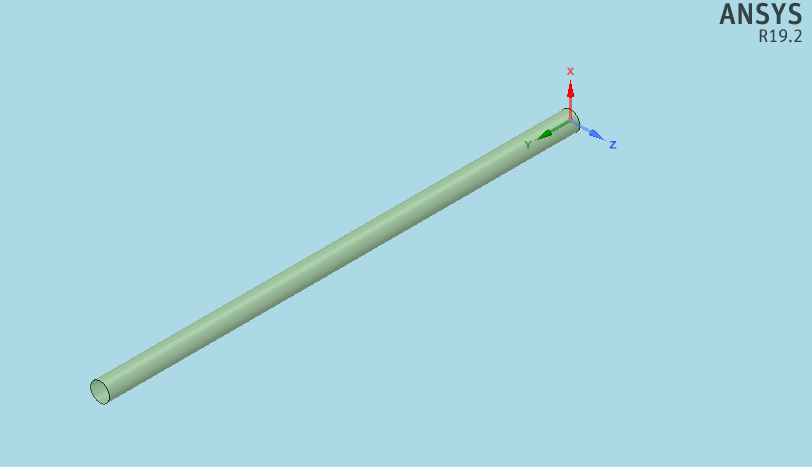
\includegraphics[width=.5\textwidth]{fig/isometric_view.png}
    \caption{Vista isométrica da geometria.}
		\label{fig:isometric}
\end{figure}

\begin{figure}[H]
    \centering
    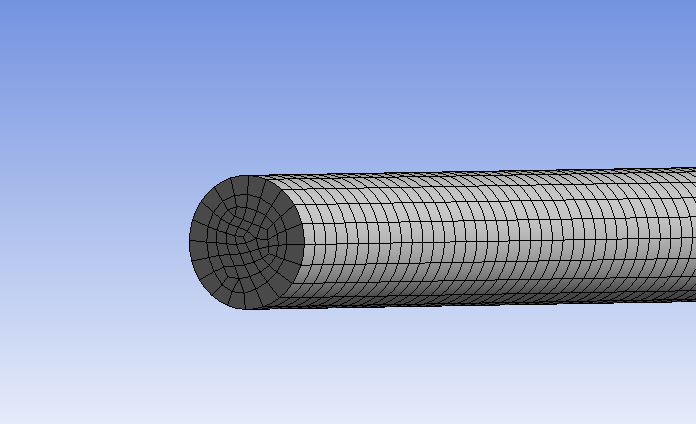
\includegraphics[width=.5\textwidth]{fig/mesh.png}
    \caption{Malha de cálculo utilizada.}
		\label{fig:isometric}
\end{figure}

Como dito anteriormente, o escoamento encontra-se na região de transição entre laminar e turbulento, portanto, é necessária a realização da análise adotando um modelo de turbulência. Para esta simulação, o modelo escolhido foi o modelo de turbulência k-epsilon. Desse modo, as informações calculadas teoricamente são utilizadas como condições de entrada para a simulação numérica. Os resultados da simulação computacional serão apresentados na tabela abaixo. 

\begin{table}[ht]
\begin{center}
\begin{tabular}{cccc} 
\hline
\textbf{Reynolds} & \textbf{Vazão volumétrica} & \textbf{Queda de Pressão} & \textbf{Tensão Cisalhante}\\
\hline
3608 &   0.001 $m^3/s$ & 3.10129 Pa & 0.02918 Pa \\
\hline
\end{tabular}
\caption{Resultados da simulação.}
\label{tbl:resultados} % spaces are big no-no withing labels
\end{center}
\end{table}

\begin{figure}[H]
    \centering
    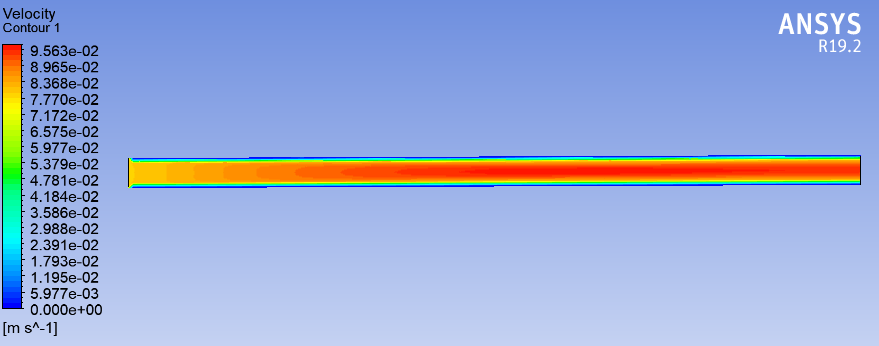
\includegraphics[width=.5\textwidth]{fig/velocity_contour_turbulent.png}
    \caption{Contorno de velocidade}
		\label{fig:isometric}
\end{figure}

\begin{figure}[H]
    \centering
    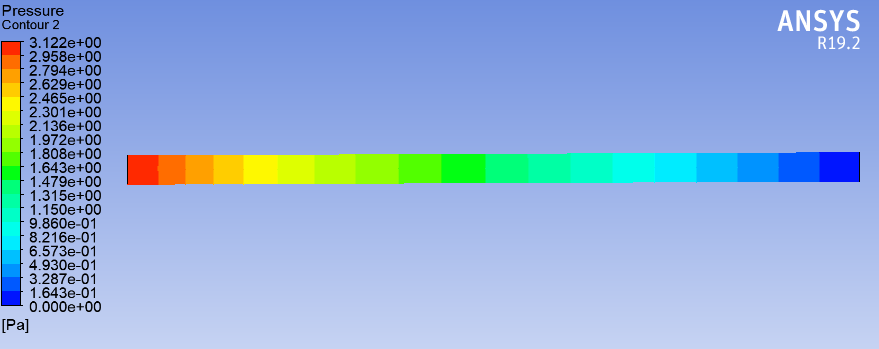
\includegraphics[width=.5\textwidth]{fig/pressure_contour_turbulent.png}
    \caption{Contorno de pressão.}
		\label{fig:isometric}
\end{figure}

\begin{figure}[H]
    \centering
    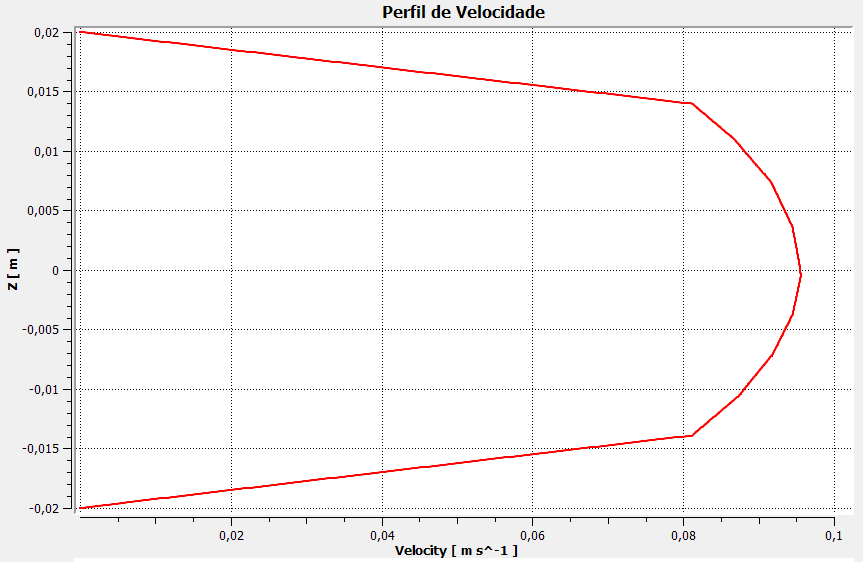
\includegraphics[width=.5\textwidth]{fig/velocity_profile_turbulent.png}
    \caption{Perfil de velocidade no meio da tubulação.}
		\label{fig:isometric}
\end{figure}

\begin{figure}[H]
    \centering
    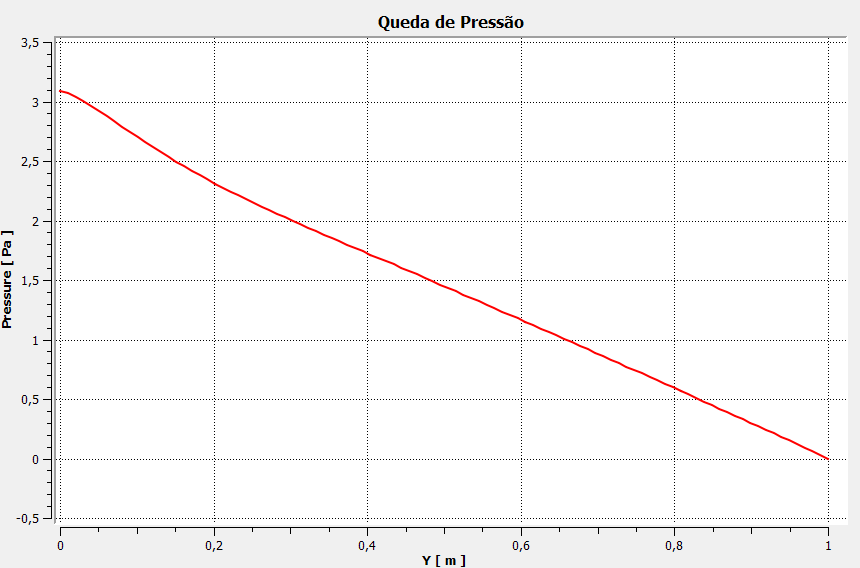
\includegraphics[width=.5\textwidth]{fig/pressure_loss_turbulent.png}
    \caption{Queda de pressão ao longo da tubulação.}
		\label{fig:isometric}
\end{figure}

Como demonstrado acima, os resultados apresentados fazendo uso do modelo de turbulência são capazes de prover uma análise tanto qualitativa quanto quantitativa. Segundo o dado teórico calculado para a queda de pressão, a taxa de erro foi de 9,4\%, a qual é plenamente aceitável para um projeto de CFD em sua segunda iteração. Desse modo, caso haja necessidade de melhorar a precisão do cálculo, é possível aprimorar a malha de cálculo utilizada.

\section{Considerações Finais}
Desse modo, foi realizado um estudo numérico de uma tubulação aplicada no bombeamento de água utilizando o código comercial Ansys CFX. Ao comparar-se os valores teóricos e numéricos com os dados experimentais do problema é possível notar uma grande discrepância nos valores da queda de pressão. Logo, conclui-se que existem erros nas dimensões da tubulação ou nas medições apresentadas para nortear a análise numérica. Por fim, a simulação numérica permitiu uma análise qualitativa e quantitativa do problema, embora, nesse contexto, aplicada a um caso simples é uma ferramenta poderosíssima no âmbito da engenharia do ponto de vista de produtividade e de custos envolvidos \cite{cfd}.

\bibliographystyle{ieeetran}
\bibliography{lib}


\end{document}
